\chapter{Anwendung}

\section{Modellierung einer Microservice-Architektur für einen Anwendungsfall}

\subsection{Vorstellung des Anwendungsfalles}

In diesem Kapitel wird eine Softwarelösung für einen Webshop modelliert. Diese Lösung soll es Kunden ermöglichen, sich zu registrieren, Bestellungen durchzuführen, diese abzuwickeln und abschließend an ein Backoffice-System zu übertragen. Zusätzlich sollen bei der Registrierung betrügerische Kunden automatisch erkannt werden. Um das Einkaufsverhalten exemplarisch zu zeigen, soll das Kaufverhalten so implementiert werden, dass Kunden so lange Käufe tätigen, bis sie zwei Bestellungen getätigt haben. Weiterhin soll der Checkout-Prozess mit einer fünfprozentigen Wahrscheinlichkeit fehlschlagen. Das Registrieren eines Kunden, die Erzeugung einer Bestellung und der erfolgreiche Checkout-Prozess sollen in Form eines Events prozessiert werden, und dieses soll dem Backoffice-System mitgeteilt werden.

\begin{figure}[ht]
\centering
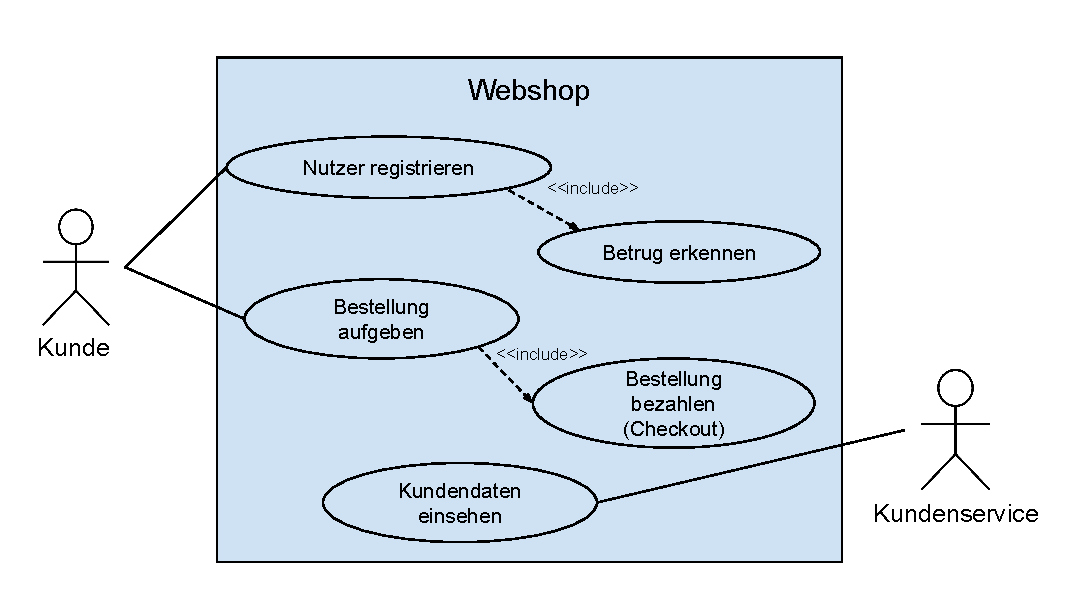
\includegraphics[height=8cm]{bilder/k6/UseCase.pdf}
\caption{Use-Case Diagramm für den Webshop-Anwendungsfall}
\end{figure}

\newpage

\subsection{Ablauf der Modellierung mit Editor}

Nach der Initialisierung des Grundmodells, wie in Kapitel 5.3 definiert, werden mit einer ContextRelationshipDescription erkannte BoundedContexts modelliert. Diesen werden Microservices und DomainModels zugewiesen. Ebenso wird ein SharedKernel \glqq Pricing\grqq{} identifiziert, welcher Teil der Kontexte \glqq Order\grqq{} und \glqq Checkout\grqq{} ist. Eine Abhängigkeit zu einer passenden Bibliothek wird ebenso modelliert. Zusätzlich werden Beziehungen zwischen den BoundedContexts entworfen. Der \glqq Backoffice\grqq-Kontext besitzt als Datensenke ein auf seinen Anwendungszweck als Datenarchiv spezialisiertes Verständnis von Kunden-, Bestellungs- und Checkout-Informationen. Dies kann in der Realität durch ein ERP-System wie SAP oder Salesforce notwendig sein. Der Kundenkontext wird als Published Language gegenüber dem Order Kontext modelliert, was durch das Veröffentlichen einer Beschreibung der Datenstruktur für Kunden umgesetzt werden könnte. Da der Order Kontext aus Gründen der Datensparsamkeit nur ein begrenztes Verständnis von den Daten hat, wird in Form einer Anticorruption Layer der Kunde in ein eigenes Modell übersetzt. Anders hingegen wird der Checkout modelliert, welcher das Modell der Bestellung übernehmen soll.

\begin{figure}[ht]
\centering
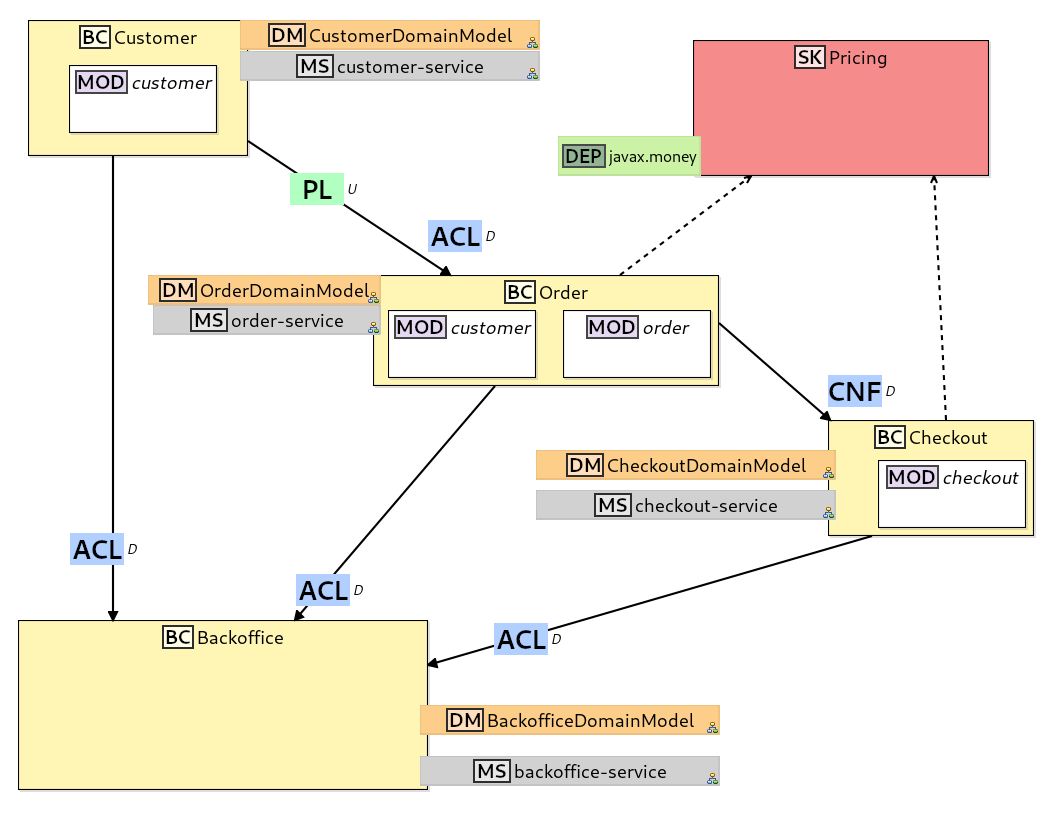
\includegraphics[width=\textwidth]{bilder/k6/1.png}
\caption{Modellierung der Bounded Contexts für den Anwendungsfall}
\end{figure}

\newpage

Nun werden die einzelnen DomainModels weiter verfeinert. Dem DomainModel des BoundedContext Order werden zwei Module, \glqq Customer\grqq{} und \glqq Order\grqq, hinzugefügt. Eine \glqq CustomerEntity\grqq{} beinhaltet die notwendigen Daten eines Kunden und wird von einer \glqq CustomerFactory\grqq{} erzeugt sowie von einem \glqq CustomerRepository\grqq{} persistiert. Dieses kann Kunden mit weniger als einer variablen Anzahl an Bestellungen finden. Ähnlich wird eine \glqq OrderEntity\grqq{} mit einem Repository und einer Factory modelliert, welche bei der Erzeugung einen Bestellwert berechnet. Ein \glqq OrderProcessService\grqq{} erzeugt Bestellungen und fordert einen Checkout-Prozess an. Zusätzlich wird das Event, das bei der Erzeugung einer Bestellung auftritt, angelegt. Das Modellieren anderer Domänen funktioniert nun konzeptionell symetrisch zu diesem Vorgehen.

\begin{figure}[ht]
\centering
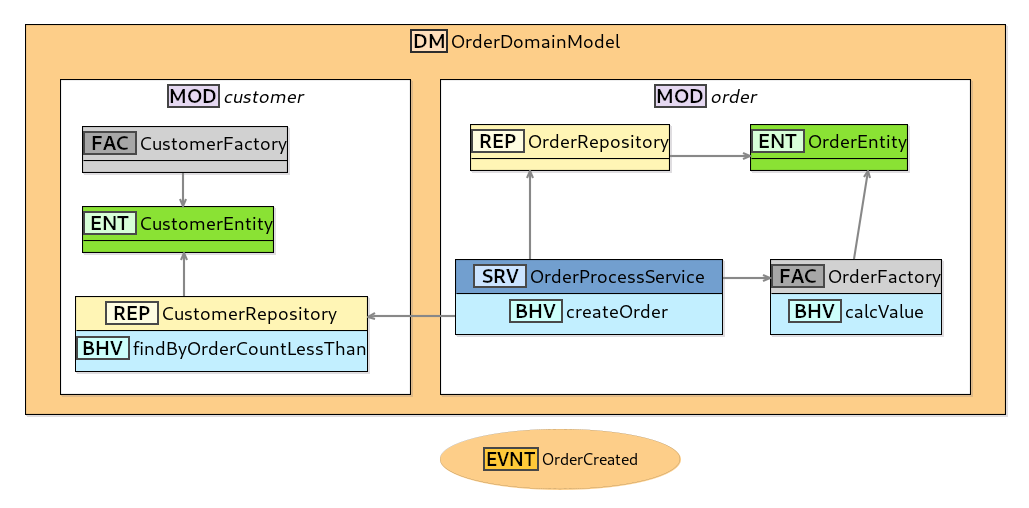
\includegraphics[width=\textwidth]{bilder/k6/3.png}
\caption{Modellierung des OrderDomainModel für den Anwendungsfall}
\end{figure}

\begin{figure}[ht]
\centering
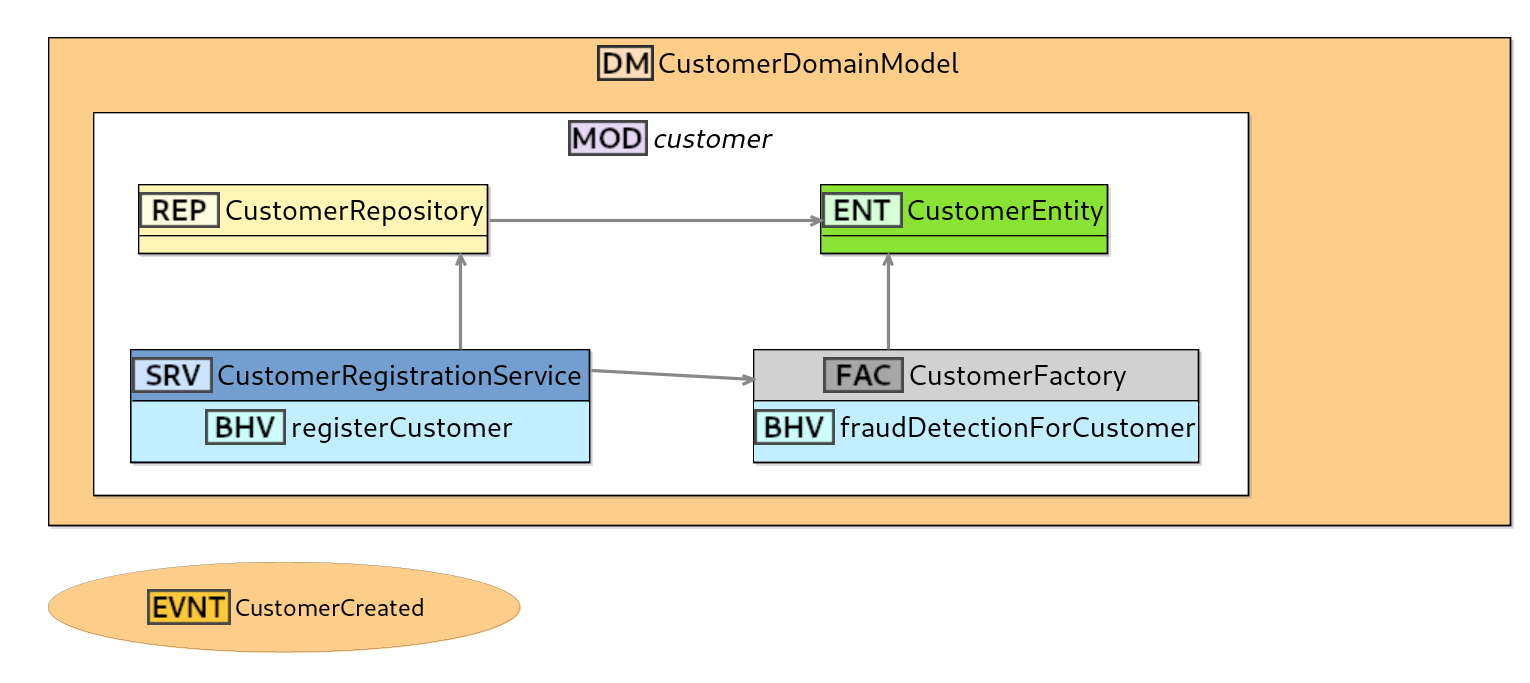
\includegraphics[width=\textwidth]{bilder/k6/extra.png}
\caption{Konzeptionell symetrische Modellierung des CustomerDomainModel}
\end{figure}


\newpage


In der Übersicht über die Microservice-Kommunikation werden nun passende Schnittstellen für die Microservices angelegt. Mittels asynchroner Schnittstellen werden über Topics Daten übertragen. Die Kommunikation zwischen Order und Checkout hingegen läuft synchron, da eine Bestellung erst abgeschlossen wird, sobald ein Checkout erfolgreich durchgeführt wurde.


\begin{figure}[ht]
\centering
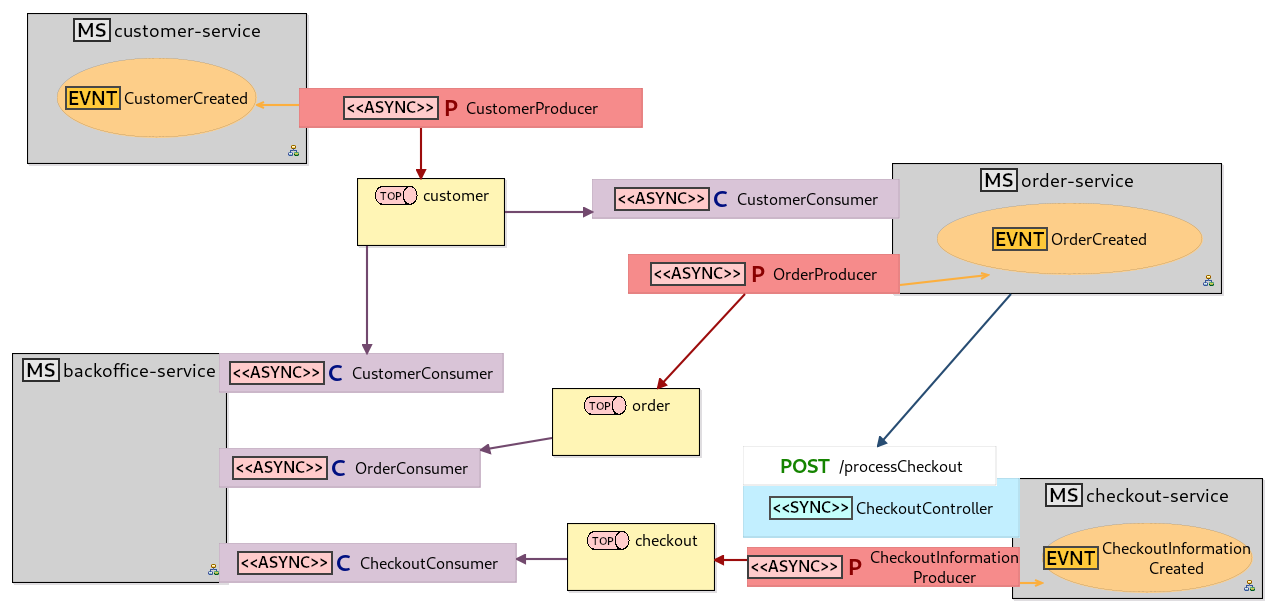
\includegraphics[width=0.95\textwidth]{bilder/k6/4.png}
\caption{Modellierung der Kommunikation zwichen Microservices für den Anwendungsfall}
\end{figure}


In den servicespezifischen Schnittstellenbeschreibungen werden die im vorherigen Modellierungsschritt definierten Schnittstellen den Modellelementen zugewiesen. Hier wird beispielsweise durch den \glqq OrderProcessService\grqq{} der Checkout-Service angefragt und mit dem \glqq OrderProducer\grqq{} das erfolgreiche Erzeugen einer Bestellung auf das im vorherigen Schritt angelegte Topic geschrieben. Weiterhin werden dem \glqq CustomerConsumer\grqq{} die passende Factory zum Erzeugen der Entities und das Repository zum Persistieren zugewiesen.

\begin{figure}[ht]
\centering
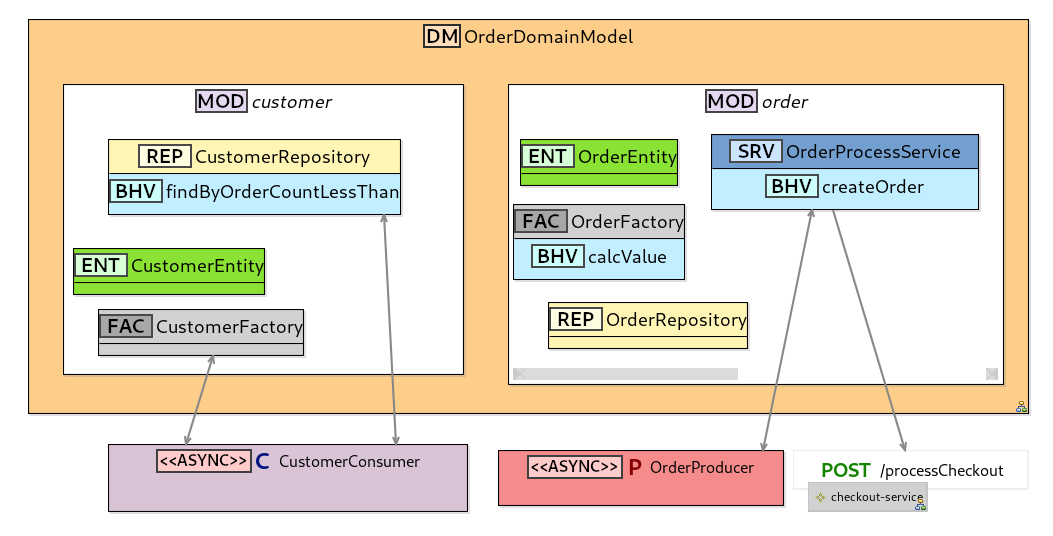
\includegraphics[width=0.95\textwidth]{bilder/k6/5.png}
\caption{Modellierung des Schnittstellen auf Serviceebene für den Anwendungsfall}
\end{figure}

\newpage

Nun kann abschließend der Cloud-Konfiguration ein Cluster hinzugefügt werden, und diesem wiederum je Service ein Deployment. Abschließend werden die Build-Konfigurationen angelegt und diesen die bereits bei der Analyse der Domäne modellierte Bibliothek \glqq javax.money\grqq{} zugewiesen.

\begin{figure}[ht]
\centering
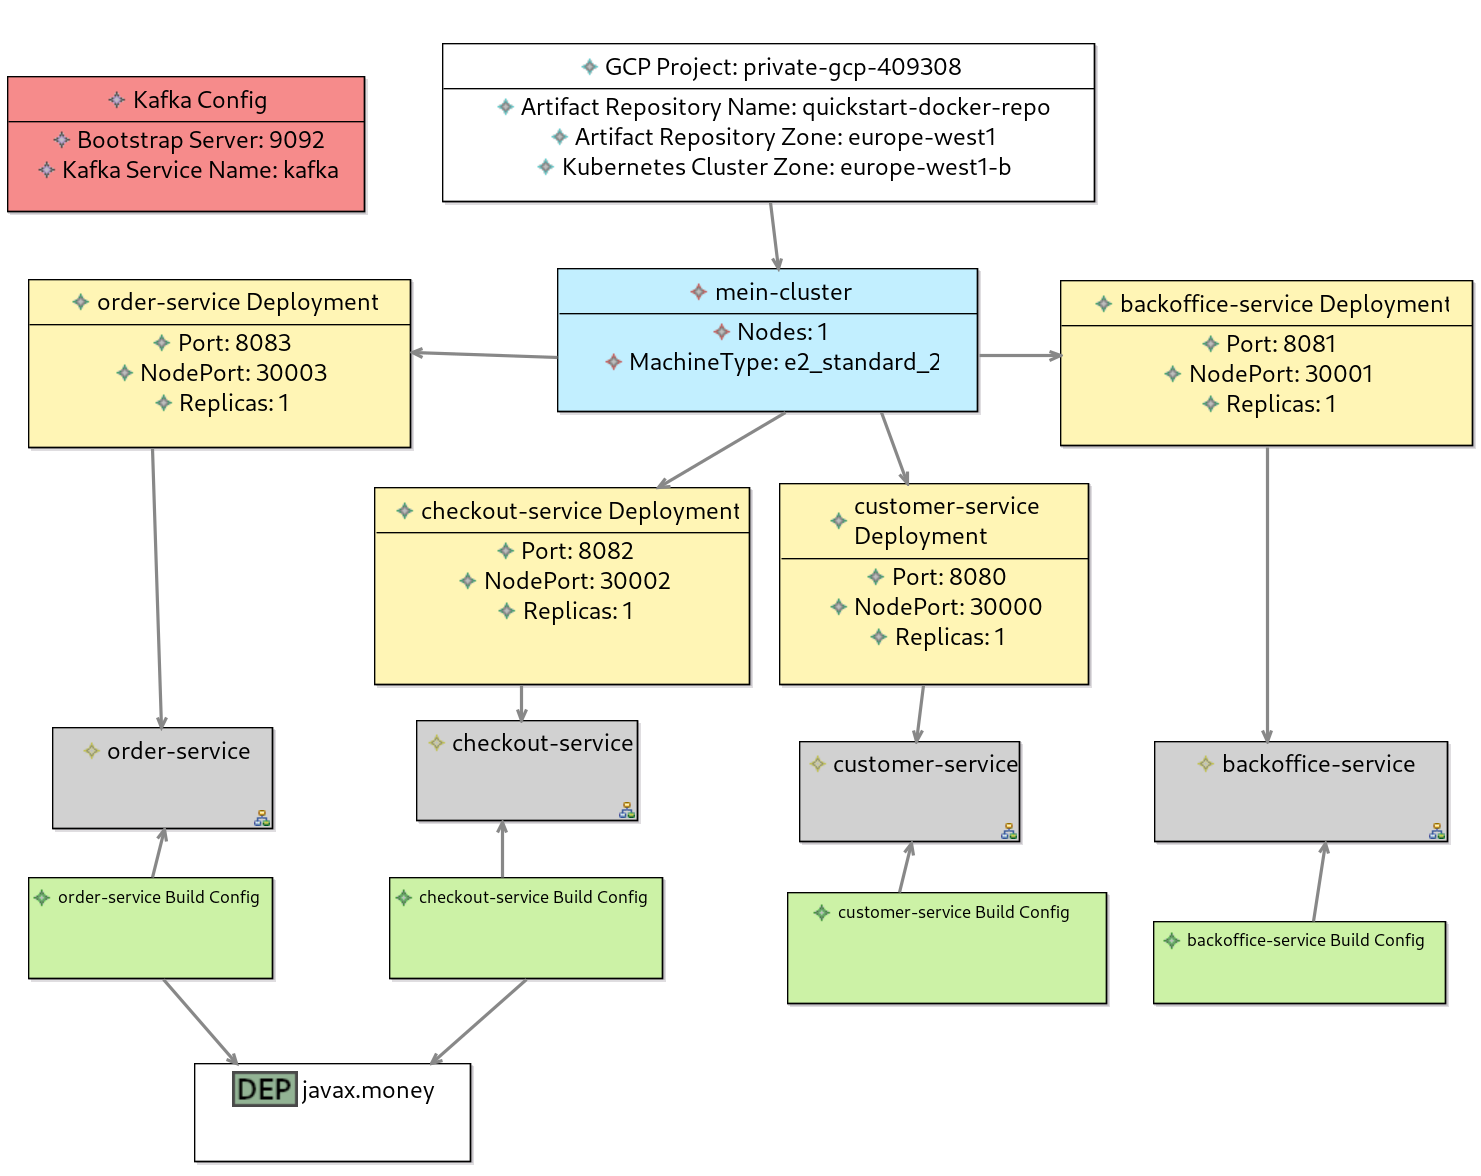
\includegraphics[width=\textwidth]{bilder/k6/6.png}
\caption{Modellierung der Infrastruktur für den Anwendungsfall}
\end{figure}

Somit wurde ein Anwendungsfall mit einer Microservice-Architektur modelliert, die die Konzepte des DDD einbezieht. Weiterhin wurden eine Ausführungsumgebung und die zur Ausführung benötigten Abstraktionen in dieses Architekturmodell einbezogen.

\newpage

\section{Inbetriebnahme}

Mit diesem Modell kann nun der dem Modell entsprechende Code generiert werden. Im Folgenden sollen die abschließenden Schritte beschrieben werden, die nun notwendig sind, um die generierten Projekte in der Cloud auszuführen.

Die modellierten Funktionalitäten müssen zunächst implementiert werden. Dies wird hier exemplarisch anhand der Methode gezeigt, die Bestellungen erzeugt.

\begin{figure}[ht]
\centering
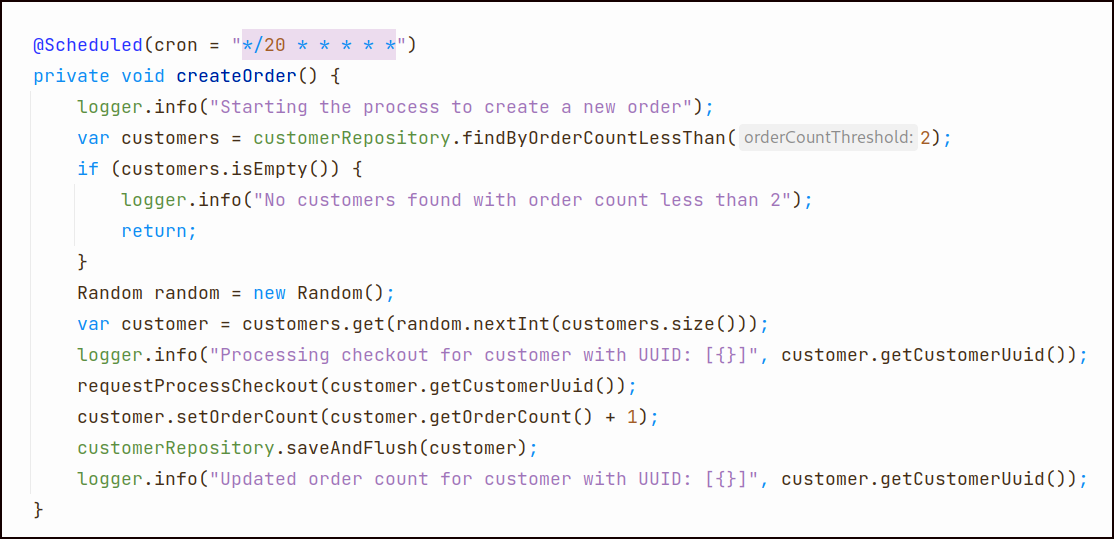
\includegraphics[width=\textwidth]{bilder/k7/1_light.png}
\caption{Implementieren von fehlenden Methoden vor der Inbetriebnahme}
\end{figure}

Weiterhin müssen Klassen attributiert werden. Im Folgenden wird ein Vergleich zwischen einer generierten Entity und einer leicht ausimplementierten Variante gezeigt.

\begin{figure}[ht]
\centering
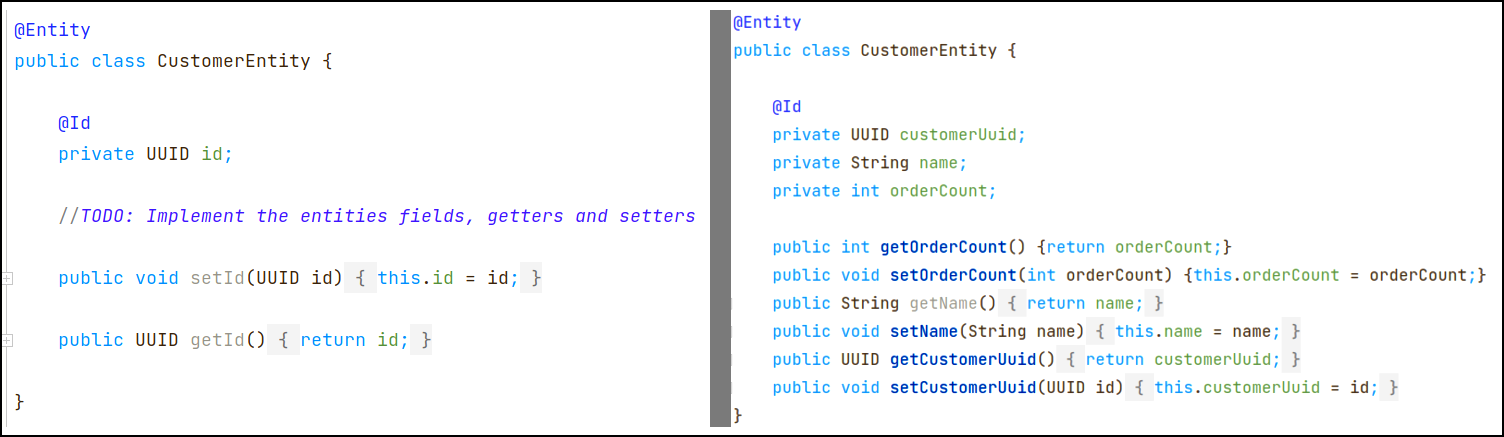
\includegraphics[width=\textwidth]{bilder/k7/2_light.png}
\caption{Implementieren von fehlenden Klassenattributen vor der Inbetriebnahme}
\end{figure}

\newpage

Um das Codegenerierungstemplate lesbar zu gestalten, wurde es durch Verwendung von Tabstopps entsprechend formatiert. Dies führt jedoch zu dem Problem, dass diese mitgeneriert werden, was zu schlecht lesbarem Code führt. Deswegen wird in einem weiteren manuellen Schritt der Code nochmals formatiert. Die folgende Abbildung zeigt exemplarisch die dadurch eingesparte Menge an Codezeilen:

\begin{figure}[ht]
\centering
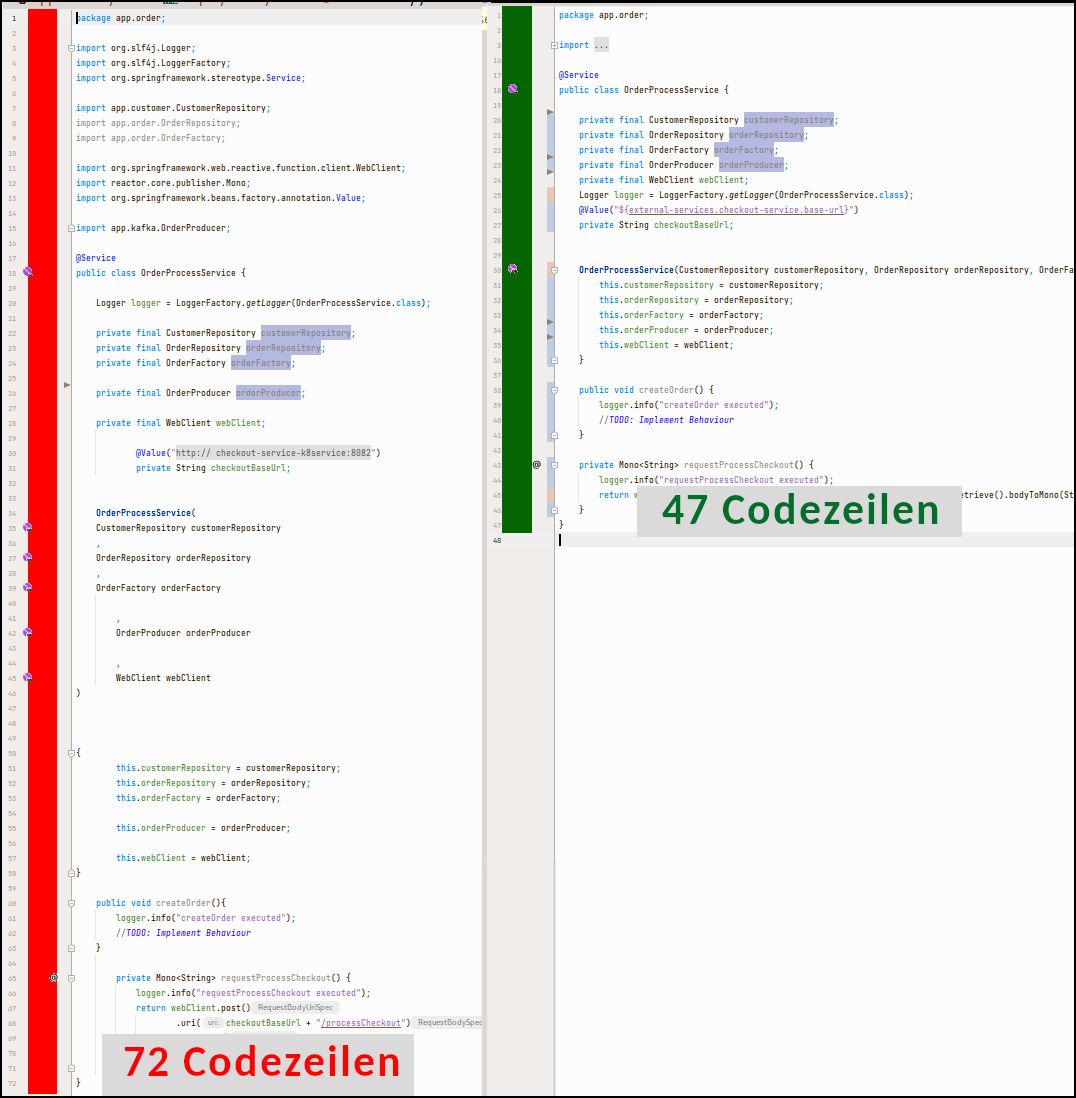
\includegraphics[width=\textwidth]{bilder/k7/3.png}
\caption{Abschließende Code-Formatierung für bessere Lesbarkeit}
\end{figure}

\newpage

Nachdem alle notwendigen Anpassungen durchgeführt wurden, können mit den generierten Bash-Skripten für die Dienste Deployments ausgeführt werden. Zu beachten ist bei den Skripten die möglicherweise notwendige Anpassung des Wurzelverzeichnisses. Dieses sollte auf das Verzeichnis verweisen, welches die generierten Dienste enthält. Durch die folgende Ausführung können dann die Dienste ausgerollt werden.

\begin{table}[h]
\centering
\small
\begin{tabular}{|c|l|}
\hline
\textbf{Schritt} & \textbf{Beschreibung}                                      \\ \hline
1                & Erzeugen von Cluster und Artifact Repository, wenn noch nicht vorhanden.               \\ \hline
2                & Whitelisten der eigenen IP                                 \\ \hline
3                & Deployment des Kafka-Images                                \\ \hline
4                & Erzeugen der Kafka-Topics                                  \\ \hline
5                & Erzeugen der Gradle-Wrapper                                \\ \hline
6                & Bauen der Images                                           \\ \hline
7                & Deployment der Services                                    \\ \hline
\end{tabular}
\caption{Deployment-Schritte für die Software}
\label{tab:deployment_steps}
\end{table}

Damit wäre die modellierte Microservice-Architektur ausgeliefert und kann sowohl über Logs beobachtet, als auch über direkte HTTP-Anfragen angesprochen werden. Somit wurde mittels eines modellgetriebenen Softwareentwicklungsansatzes eine lauffähige Microservice-Architektur modelliert, entwickelt und bereitgestellt.

Der vollständige Quellcode, der das in dieser Arbeit konzipierte Metamodell, die Definition der konkreten Syntax, das Generierungstemplate und verschiedene Beispielprojekte umfasst, liegt dieser Arbeit bei. Weiterhin ist dieser öffentlich in einem GitHub-Repository \cite{github} einsehbar (Stand: 30. Januar 2024).